% Options for packages loaded elsewhere
\PassOptionsToPackage{unicode}{hyperref}
\PassOptionsToPackage{hyphens}{url}
%
\documentclass[12pt
]{article}
\usepackage{amsmath,amssymb}
\usepackage{iftex}
\ifPDFTeX
  \usepackage[T1]{fontenc}
  \usepackage[utf8]{inputenc}
  \usepackage{textcomp} % provide euro and other symbols
\else % if luatex or xetex
  \usepackage{unicode-math} % this also loads fontspec
  \defaultfontfeatures{Scale=MatchLowercase}
  \defaultfontfeatures[\rmfamily]{Ligatures=TeX,Scale=1}
\fi
\usepackage{lmodern}
\ifPDFTeX\else
  % xetex/luatex font selection
\fi
% Use upquote if available, for straight quotes in verbatim environments
\IfFileExists{upquote.sty}{\usepackage{upquote}}{}
\IfFileExists{microtype.sty}{% use microtype if available
  \usepackage[]{microtype}
  \UseMicrotypeSet[protrusion]{basicmath} % disable protrusion for tt fonts
}{}
\makeatletter
\@ifundefined{KOMAClassName}{% if non-KOMA class
  \IfFileExists{parskip.sty}{%
    \usepackage{parskip}
  }{% else
    \setlength{\parindent}{0pt}
    \setlength{\parskip}{6pt plus 2pt minus 1pt}}
}{% if KOMA class
  \KOMAoptions{parskip=half}}
\makeatother
\usepackage{xcolor}
\usepackage[margin=1in]{geometry}
\usepackage{graphicx}
\makeatletter
\def\maxwidth{\ifdim\Gin@nat@width>\linewidth\linewidth\else\Gin@nat@width\fi}
\def\maxheight{\ifdim\Gin@nat@height>\textheight\textheight\else\Gin@nat@height\fi}
\makeatother
% Scale images if necessary, so that they will not overflow the page
% margins by default, and it is still possible to overwrite the defaults
% using explicit options in \includegraphics[width, height, ...]{}
\setkeys{Gin}{width=\maxwidth,height=\maxheight,keepaspectratio}
% Set default figure placement to htbp
\makeatletter
\def\fps@figure{htbp}
\makeatother
\setlength{\emergencystretch}{3em} % prevent overfull lines
\providecommand{\tightlist}{%
  \setlength{\itemsep}{0pt}\setlength{\parskip}{0pt}}
\setcounter{secnumdepth}{-\maxdimen} % remove section numbering
\let\oldsection\section
\renewcommand{\section}[1]{\clearpage\oldsection{#1}}
  \def\tightlist{}
\ifLuaTeX
  \usepackage{selnolig}  % disable illegal ligatures
\fi
\IfFileExists{bookmark.sty}{\usepackage{bookmark}}{\usepackage{hyperref}}
\IfFileExists{xurl.sty}{\usepackage{xurl}}{} % add URL line breaks if available
\urlstyle{same}
\hypersetup{
  hidelinks,
  pdfcreator={LaTeX via pandoc}}

\author{}
\date{}

\begin{document}

\section{Review Test 1}\label{review-test-1}

\begin{enumerate}
\def\labelenumi{\arabic{enumi}.}
\item
  Evaluate
  \[\lim_{h \rightarrow 0}\dfrac{\sec(3(x + h)) - \sec(3x)}{h}\]

  \begin{enumerate}
  \def\labelenumii{\alph{enumii}.}
  \setcounter{enumii}{1}
  \tightlist
  \item
    \(3\sec(3x)\tan(3x)\)
  \item
    0
  \item
    \(\sec^{2}(3x)\)
  \item
    \(3\cot(3x)\)
  \item
    nonexistent
  \end{enumerate}
\item
  \[f(x) = \left\{ \begin{matrix}
  2x + 3b\text{ if }x \leq 2 \\
  3ax^{2}\text{ if }x > 2
  \end{matrix} \right.\ \] Let \(f\) be the function given above. What
  are all values of \(a\) and \(b\) for which \(f\) is differentiable at
  \(x = 2\) ?

  \begin{enumerate}
  \def\labelenumii{\alph{enumii}.}
  \tightlist
  \item
    \(a = \dfrac{1}{6} \quad b = \dfrac{-2}{3}\)
  \item
    \(\quad a = \dfrac{1}{4}\) and \(b = \dfrac{1}{2}\)
  \item
    \(\quad a = \dfrac{1}{4}\) and \(b\) is any real number
  \item
    \(a = b + 2\), where \(b\) is any real number
  \item
    There are no such values of \(a\) and \(b\)
  \end{enumerate}
\item
  If the function \(f\) is continuous for all real numbers and if
  \(f(x) = \dfrac{x^{2} - 25}{x - 5}\) when \(x \neq 5\), then
  \(f( 5 ) =\)

  \begin{enumerate}
  \def\labelenumii{\alph{enumii}.}
  \tightlist
  \item
    10
  \item
    5
  \item
    25
  \item
    -5
  \item
    -1
  \end{enumerate}
\item
  Evaluate \[\lim_{x \rightarrow e}\dfrac{\ln 2x - \ln 2}{x - e}\]

  \begin{enumerate}
  \def\labelenumii{\alph{enumii}.}
  \tightlist
  \item
    \(\dfrac{1}{e}\)
  \item
    1
  \item
    \(e\)
  \item
    Nonexistent
  \end{enumerate}
\item
  \[\lim_{x \rightarrow 0}\dfrac{1 - \cos x}{x^{2} + \sin(4x)} =\]

  \begin{enumerate}
  \def\labelenumii{\alph{enumii}.}
  \tightlist
  \item
    0
  \item
    2
  \item
    1
  \item
    3
  \end{enumerate}
\item
  \[f(x) = \left\{ \begin{matrix}
  x^2\text{ for }x < 3 \\
  \dfrac{1}{3}\text{ for }x \geq 3
  \end{matrix} \right.\ \] If \(f\) is the function defined above, then
  \(\displaystyle \int_{- 2}^{4}f(x)dx\) is

  \begin{enumerate}
  \def\labelenumii{\alph{enumii}.}
  \tightlist
  \item
    12
  \item
    \(\dfrac{15}{2}\)
  \item
    \(\dfrac{17}{2}\)
  \item
    undefined
  \end{enumerate}
\item
  \[\displaystyle \int_{0}^{3}\dfrac{x^{2} + 5x + 6}{x + 2}dx =\]

  \begin{enumerate}
  \def\labelenumii{\alph{enumii}.}
  \tightlist
  \item
    \(\dfrac{27}{2}\)
  \item
    \(3 + 2\ln 2\)
  \item
    \(\dfrac{15}{2} + 2\ln 2\)
  \item
    \(\dfrac{15}{2} + 2\ln 3\)
  \end{enumerate}
\item
  \[\displaystyle \int \dfrac{\cos{\left(\sqrt{x} + 1\right)}}{\sqrt x}\; dx =\]

  \begin{enumerate}
  \def\labelenumii{\alph{enumii}.}
  \tightlist
  \item
    \(2\sin \left(\sqrt{x} + 1\right) + C\)
  \item
    \(e^{x}\sin\left( e^{x} + 1 \right) + C\)
  \item
    \(e^{x}\sin\left( e^{x} + x \right) + C\)
  \item
    \(\dfrac{1}{2}\cos^{2}\left( e^{x} + 1 \right) + C\)
  \end{enumerate}
\item
  \[\displaystyle \int\dfrac{2x}{x^{2} + 9}dx =\]

  \begin{enumerate}
  \def\labelenumii{\alph{enumii}.}
  \tightlist
  \item
    \(\ln (x^2+9)\)
  \item
    \(\dfrac{1}{2\left( x^{2} - 4 \right)} + C\)
  \item
    \(\dfrac{1}{2}\ln\left| x^{2} - 4 \right| + C\)
  \item
    \(2\ln\left| x^{2} - 4 \right| + C\)
  \item
    \(\dfrac{1}{2}\arctan\left( \dfrac{x}{2} \right) + C\)
  \end{enumerate}
\item
  The function \(g\) is continuous on the closed interval
  \(\lbrack 2,10\rbrack\). If \(\displaystyle \int_{9}^{1} g(x)dx = 25\)
  and \(\displaystyle \int_{1}^{5}\dfrac{1}{2}g(x)dx = - 12\), then
  \(\displaystyle \int_{5}^{9} g(x)dx =\)

  \begin{enumerate}
  \def\labelenumii{\alph{enumii}.}
  \tightlist
  \item
    -1
  \item
    62
  \item
    95
  \item
    190
  \end{enumerate}
\item
  Using the substitution \(u = 2x^{2} + 1\), the integral
  \(\displaystyle \int_{2}^{4}2x\left( 2x^2+1 \right)^{3}dx\) is equal
  to which of the following?

  \begin{enumerate}
  \def\labelenumii{\alph{enumii}.}
  \tightlist
  \item
    \(\displaystyle \frac{1}{2} \int_9^{33} u^3 \; du\)
  \item
    \(\displaystyle \int_{- 2}^{13}u^{5}du\)
  \item
    \(\dfrac{1}{2}\displaystyle \int_{- 2}^{13}u^{5}du\)
  \item
    \(2\displaystyle \int_{- 2}^{13}u^{5}du\)
  \item
    \(\displaystyle \int_{- 1}^{4}u^{5}du\)
  \end{enumerate}
\item
  \[\displaystyle \int\dfrac{9x+1}{(2x + 1)(x - 3)}dx\]

  \begin{enumerate}
  \def\labelenumii{\alph{enumii}.}
  \tightlist
  \item
    \(\ln | 2x+1 | + 4 \ln |x-3| + C\)
  \item
    \(3\ln|2x - 3| + 2\ln|x + 2| + C\)
  \item
    \(3\ln|2x - 3| - 2\ln|x + 2| + C\)
  \item
    \(- \dfrac{6}{(2x - 3)^{2}} - \dfrac{2}{(x + 2)^{2}} + C\)
  \end{enumerate}
\item
  \[\displaystyle \int\dfrac{1}{x^{2} - 16x + 80}dx =\]

  \begin{enumerate}
  \def\labelenumii{\alph{enumii}.}
  \tightlist
  \item
    \(\dfrac{1}{4} \arctan \left( \dfrac {x-8}{4} \right)\)
  \item
    \(\arctan\left( \dfrac{x - 5}{9} \right) + C\)
  \item
    \(\dfrac{1}{3}\arctan\left( \dfrac{x - 5}{3} \right) + C\)
  \item
    \(3\arctan\left( \dfrac{x - 5}{3} \right) + C\)
  \end{enumerate}
\item
  The graph of a piecewise linear function \(f\) is given.

  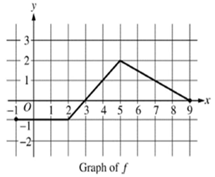
\includegraphics[width=2.23958in,height=1.84375in]{media/image1.png}

  What is the value of
  \(\displaystyle \int_{1}^{7}\left( 4f(x) - 1 \right)dx\) ?

  \begin{enumerate}
  \def\labelenumii{\alph{enumii}.}
  \tightlist
  \item
    8
  \item
    9.5
  \item
    27.5
  \item
    47
  \item
    48.5
  \end{enumerate}
\item
  Evaluate \[\displaystyle \int_{1}^{\infty}xe^{-(x^{2}-1)}dx\]

  \begin{enumerate}
  \def\labelenumii{\alph{enumii}.}
  \tightlist
  \item
    \(\dfrac{e}{2}\)
  \item
    \(\dfrac{1}{2e}\)
  \item
    \(\dfrac{1}{e}\)
  \item
    \(\dfrac{2}{e}\)
  \item
    divergent
  \end{enumerate}
\item
  Integrate \[\int x^3 e^{2x} \; dx\]

  \begin{enumerate}
  \def\labelenumii{\alph{enumii}.}
  \tightlist
  \item
    \(\dfrac{1}{8} e^{2 x} \left(4 x^3-6 x^2+6 x-3\right) + C\)
  \end{enumerate}
\end{enumerate}

\end{document}
